\chapter{Etat de l'art}
\dochaptoc
\label{ch-chapter_2}

%
\section{Formulation du problème d'inpainting}

\subsection{Présentation générale}

Un grand nombre de méthodes ont émergées au cours de la dernière décennie afin de reconstruire une image avec une grande précision en ne disposant que d'une acquisition partielle. Plus généralement, beaucoup de problèmes inverses ont été intensément étudiés sous le prisme de l'acquisition comprimée. L'acquisition comprimée est un framework général qui fournit des méthodes de restauration avec des garanties théoriques pour les problèmes inverses linéaires sous-déterminés. Ces travaux d'Emmanuel Candès, Justin Romberg, Terence Tao et David Donoho~\cite{candes2006near, candes2006stable, donoho2006compressed} ont révolutionné le domaine du traitement du signal. Ceux-ci ont démontré qu'une image acquise avec une fréquence d'échantillonnage inférieure à celle de Nyquist pouvait être restaurée de manière exacte sous certaines conditions (dont une spécifiant que les données doivent être parcimonieuses dans une certaine base). Le paradigme de l'acquisition comprimée requiert que les données soient projetées sur $n$ sous-espaces aléatoires, avec $n$ très petites devant la taille des données. Cette technique a été appliqué avec succès dans de nombreux domaines incluant l'IRM~\cite{boyer_algorithm_2014}, l'imagerie ultrasonique~\cite{quinsac_bayesian_2011}, l'astronomie~\cite{bobin_compressed_2008} ou la tomographie~\cite{binev2012compressed, jacob2019MM, jacob2018MM} en microscopie. %
%
Ces résultats ont rendu populaire les problèmes inverses visant à compléter une image à partir d'une acquisition spatialement incomplète. Ces méthodes sont appelées techniques de \emph{complétion} ou encore d'\emph{inpainting}\footnote{Le terme d'inpainting a été introduit par les travaux de Bertalmio \textit{et al.}~\cite{bertalmio2000image} en référence aux techniques de restauration en art. En effet, leur modèle est basé sur l'observation du travail effectué par les artistes employés par les musés pour restaurer les vielles peintures.}. Il s'agit d'un domaine de recherche très actif en microscopie \gls{stem}~\cite{beche2016compressed,stevens2014potential} et \gls{sem}~\cite{anderson2013sparse} entre autres.

L'inpainting regroupe cependant deux situations distinctes nécessitant des techniques distinctes, comme le montre la \cref{fig-inpainting}. D'une part, l'information peut être fortement structurée, comme c'est le cas en retouche photographique où un élément (personne, objet) doit être supprimé d'une prise de vue~\cite{criminisi2004region}. Les \crefrange{fig-inpainting-a}{fig-inpainting-c} montrent un exemple de complétion pour des données structurées. Nous retrouvons également dans cette classe la correction de données aberrantes apparues suite à un dysfonctionnement du capteur~\cite{zhang2013hyperspectral}. D'autre part, l'acquisition peut être volontairement lacunaire pour des raisons de compression ou de préservation de l'échantillon (comme dans notre cas), l'information est alors répartie. Les \crefrange{fig-inpainting-d}{fig-inpainting-f} montrent un exemple de cette situation.

\begin{figure}
    \centering
    \subfigure[\label{fig-inpainting-a}]{
        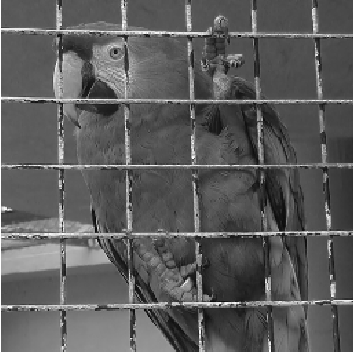
\includegraphics[width=0.25\textwidth]{img/chapitre3/figure1/initial-2.png}}\hspace{1em}
    \subfigure[\label{fig-inpainting-b}]{
        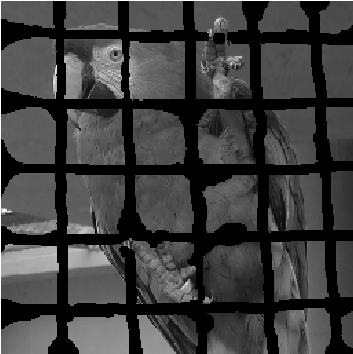
\includegraphics[width=0.25\textwidth]{img/chapitre3/figure1/mask-2.png}}\hspace{1em}
    \subfigure[\label{fig-inpainting-c}]{
        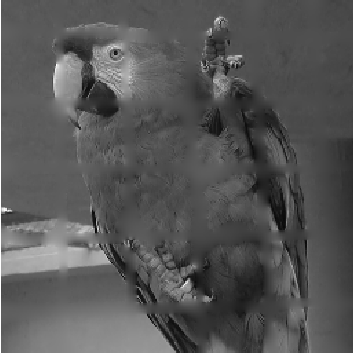
\includegraphics[width=0.25\textwidth]{img/chapitre3/figure1/final-2.png}}\\
    %
    \subfigure[\label{fig-inpainting-d}]{
        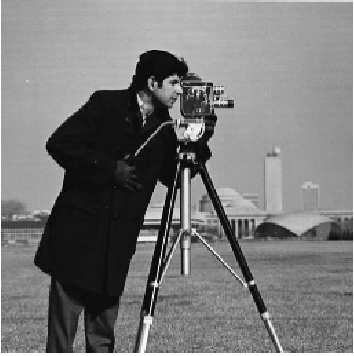
\includegraphics[width=0.25\textwidth]{img/chapitre3/figure2/initial.png}}\hspace{1em}
    \subfigure[\label{fig-inpainting-e}]{
        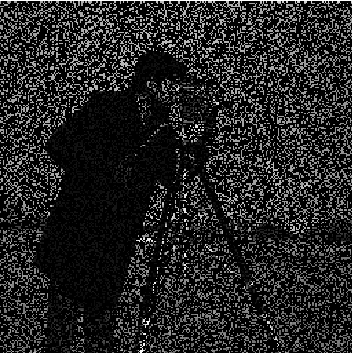
\includegraphics[width=0.25\textwidth]{img/chapitre3/figure2/mask.png}}\hspace{1em}
    \subfigure[\label{fig-inpainting-f}]{
        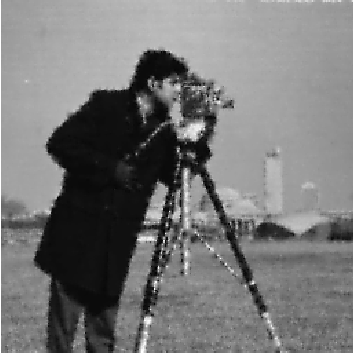
\includegraphics[width=0.25\textwidth]{img/chapitre3/figure2/final.png}}
    \caption{Exemple d'inpainting extrait de~\protect\cite{peyre2011numerical}. \protect\subref{fig-inpainting-a} Exemple d'image destinée à la retouche photographique. \protect\subref{fig-inpainting-b} Les pixels composant la grille sont enlevés de l'image. \protect\subref{fig-inpainting-c} Résultat après inpainting : la grille est enlevée de l'image. \protect\subref{fig-inpainting-d} Exemple d'acquisition complète. \protect\subref{fig-inpainting-e} La même image acquise partiellement. \protect\subref{fig-inpainting-f} Résultat après inpainting.
        \protect\label{fig-inpainting}} 
\end{figure}

La technique d'inpainting est généralement associée à la reconstruction d'images 2D, mais elle s'étend au-delà pour les images multi-dimensionnelles dont une partie des voxels (l'équivalent des pixels pour une image multi-dimensionnelle) sont manquants.
%
La stratégie d'acquisition partielle décrite à la \cref{sec-ech-sensibles} s'inscrit dans ce contexte. En effet, la sonde ne visite qu'une partie de l'échantillon en suivant un chemin généralement aléatoire. Il en résulte des données spatialement sous-échantillonées que les techniques d'inpainting peuvent compléter.
%
Notons également que ce schéma d'acquisition spatial ne s'accompagne pas d'un sous-échantillonnage spectral puisque, pour chaque position spatiale, le spectromètre \gls{eels} sépare simultanément toutes les pertes d'énergie conduisant à une acquisition complète du spectre. Il en résulte que les données issues d'une telle stratégie sont \emph{fortement structurées}.


\subsection{Problème direct et inverse}

Notons $\gls{X}\in\mathbb{R}^{\gls{M}\times\gls{P}}$ les données \gls{eels} inconnues à retrouver où \gls{P} est le nombre de pixels et \gls{M} est le nombre de canaux. %
%
Comme expliqué à la \cref{sec-ech-sensibles}, faire l'acquisition complète du spectre-image \gls{X} n'est pas toujours possible dû à la détérioration introduite par le faisceau d'électron sur l'échantillon. Pour empêcher cela, la zone d'intérêt ne peut être échantillonné qu'à certaines positions spatiales. Ainsi, les spectres complets sont acquis en \gls{N} positions parmi \gls{P}, il en résulte un rapport d'échantillonnage $\gls{r}=\gls{N}/\gls{P}$ et l'ensemble des index des \gls{N} positions spatiales visitées est noté \gls{I}. %

D'autre part, nous avons vu à la \cref{sec-prop-eels} que le bruit attaché aux données est le mélange de plusieurs contributions dont le modèle statistique diffère. Il en résulte que quantifier chacune de ces contribution est complexe en pratique et les modèles classiquement retenu dans la littérature sont les bruits poissonien~\cite{egerton2011electron, mevenkamp2015poisson, stevens2018apl} et gaussien~\cite{stevens2014potential, binev2012compressed}. Dans ce manuscrit, nous choisirons de modéliser la détérioration des données avec un bruit indépendant, additif, gaussien et blanc. Deux raisons principales expliquent ce choix :
\begin{itemize}
    \item puisque les différentes composantes de ce mélange sont difficile à quantifier, nous préférons utiliser le bruit gaussien plus simple,
    \item des expériences ont été réalisées avec un bruit poissonien seul~\cite{Monier2020SuppNum} et aucune différence notable n'a été observée par rapport à un modèle gaussien.
\end{itemize}
De plus, si une composante poissonienne émerge particulièrement, des techniques de stabilisation de variance comme la transformée de Anscombe~\cite{anscombe1948transformation} convertissent le bruit poissonien en un bruit gaussien.

Finalement, la matrice observée $\gls{Y}\in\mathbb{R}^{\gls{M}\times\gls{N}}$ peut être décrite par le modèle direct suivant :
\begin{equation}
    \gls{Y} = \gls{X}_{\gls{I}} + \gls{B}
\end{equation}
où $\gls{X}_{\gls{I}}$ est la matrice réalisée en concaténant les colonnes de \gls{X} indexées par \gls{I} et \gls{B} est un terme résiduel associé à l'erreur de modèle et le bruit d'acquisition. Les éléments de \gls{B} sont supposés être indépendants et identiquement distribués selon une loi gaussienne centrée d'écart type \gls{sig}.

Le problème de reconstruction consiste à restituer une image complète (et possiblement débruitée) \gls{X} à partir de \gls{Y}. Cependant, cette tâche est mal posée puisque le nombre de paramètres \gls{P}\gls{M} est supérieur au nombre d'observations \gls{N}\gls{M} et la suite de ce chapitre étudiera les approches possibles pour résoudre ce problème inverse.

%
\section{Les différentes classes d'inpainting}

Les techniques de reconstructions classiquement rencontrées dans la littérature vont être présentées dans cette section. Elles ont été classées en quatre sections : les techniques d'interpolation, les techniques de \gls{mc} régularisés, les techniques par diffusion et les techniques par patch.

\subsection{Les techniques d'interpolation}

\paragraph{Présentation du problème d'interpolation} Définissons un ensemble de points $(p_k)_{1\leq k\leq K}$ appartenant à un espace Euclidien de dimension $n$ (typiquement $\mathbb{R}^n$) et un ensemble de valeurs associées $(f(p_k))_{1\leq k\leq K}$ avec $f:X\rightarrow \mathbb{R}$ la fonction à interpoler. Le problème d'interpolation consiste à déterminer les valeurs prises par $f$ en un ensemble de points $(q_k)_{1\leq k\leq K}$ quelconques de $X$.
%
Ce problème est défini que l'information soit structurée ou non. Dans notre cas, nous devons considérer nos données comme un cube dont certains voxels sont manquant. L'étape d'interpolation consiste à compléter les valeurs prises par l'image en ces points.
%
Ce problème est facile en 1D et reste simple à condition que les points $(p_k)_{1\leq k\leq K}$ soient régulièrement disposés dans l'espace. Dans le cas d'un ensemble de points irrégulièrement répartis (comme c'est le cas ici), l'espace doit être découpé en éléments de base, puis interpolée sur ces éléments. Par exemple, en 2D, la surface peut être découpée en triangles. Afin d'introduire cette technique qui servira de référence dans la suite, le diagramme de Voronoi et la triangulation de Delaunay vont être succinctement définis.


\begin{marginfigure}
    \centering
    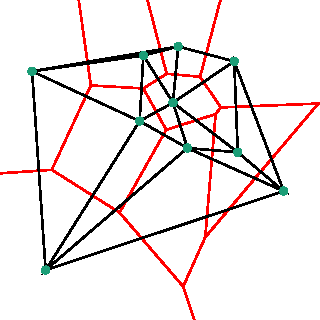
\includegraphics[]{img/chapitre3/figure3/Voronoi.pdf}
    \caption{Supperposition d'un diagramme de Voronoi (en rouge) et de sa triangulation de Delaunay (en noir). Le réseau de points est en vert.}
    \label{fig-voronoi}
\end{marginfigure}
\paragraph{Diagrammes de Voronoi et triangulation de Delaunay} Afin d'introduire les techniques d'interpolation, deux outils mathématiques simples et complémentaires seront nécessaires. Le premier, appelé diagramme de Voronoi~\cite{cazals2006delaunay}, est défini pour un ensemble de points comme suit.
\begin{mydef}[Diagramme de Voronoi]
    Soit $X$ un espace métrique de distance $d$ et $(p_k)_{1\leq k\leq K}$ un ensemble de $K$ points de $X$. La cellule de Voronoi $R_k$ associée au point $p_k$ est l'ensemble des points de $X$ plus proches de $p_k$ que de tout autre point $p_j$ pour $j$ différent de $k$. En d'autre termes, si $d(p_k, p_j)$ désigne la distance entre $p_k$ et $p_j$, nous avons
    \[R_k=\{x\in X | d(x, p_k) \leq d(x, p_j) \ \forall j\neq k\}.\]
    Le diagramme de Voronoi est définit comme l'ensemble des cellules $(R_k)_{1\leq k\leq K}$.
\end{mydef}
Le diagramme de Voronoi se visualise bien si $X$ est un espace euclidien de dimension 2 et cette notion est illustrée en rouge à la~\cref{fig-voronoi}. Une problématique communément associée à ce graphe est la \emph{triangulation} qui consiste à découper un plan en une collection de triangles. En effet, la triangulation de Delaunay~\cite{cazals2006delaunay} d'un ensemble discret de points est le graphe dual du diagramme de Voronoi et se définit comme suit.
\begin{marginfigure}
    \centering
    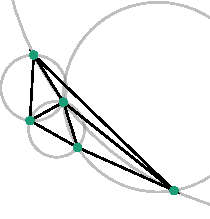
\includegraphics[]{img/chapitre3/figure3/Delaunay.pdf}
    \caption{Superposition d'un ensemble de points (en vert), de sa triangulation de Delaunay (en noir) et des cercles circonscrit à chaque triangle (en gris).}
    \label{fig-delaunay}
\end{marginfigure}
\begin{mydef}[Triangulation de Delaunay]
    Soit $P=(p_k)_{1\leq k\leq K}$ un ensemble de points appartenant à un espace Euclidien de dimension $n$. Une triangulation de Delaunay $\mathrm{DT(P)}$ est une triangulation telle qu'aucun point de $P$ ne se trouve dans l'hypersphère circonscrite d'un simplex de $\mathrm{DT(P)}$.
\end{mydef}
Notons qu'une hypersphère circonscrite (resp. un simplex) est la généralisation du cercle circonscrit (resp. du triangle) en dimension quelconque. La triangulation de Delaunay est illustrée en noir à la \cref{fig-voronoi} et les cercles circonscrit associés à chaque triangle sont mis en évidence pour un ensemble de point réduit à la \cref{fig-delaunay}. Ces deux outils vont servir à présent pour définir les techniques d'interpolation classiques.


\paragraph{Interpolation par \Glsentrylong{ppv}} L'interpolation par \gls{ppv} est la technique d'interpolation la plus simple et la moins coûteuse. Elle consiste à associer à chaque point à interpoler la valeur prise par $f$ au point échantillonné $p_{k}$ le plus proche. Cela consiste à associer $f(p_{k})$ à tout point $x$ appartenant à la cellule de Voronoi de $p_{k}$. Cette méthode, bien que très peu coûteuse, est aussi la moins efficace puisque la fonction interpolée est constante par morceaux, ce qui entraîne une erreur de reconstruction élevée. Cela est particulièrement visible sur l'exemple d'interpolation \gls{ppv} donné aux figures \ref{fig-interpolation-a} et \ref{fig-interpolation-d} puisque les cellules de Voronoi apparaissent clairement sur l'image tandis que la fonction interpolée est constante par morceaux. %
\begin{marginfigure}
    \centering
    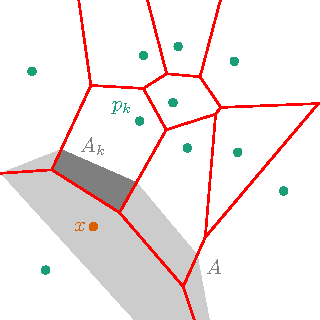
\includegraphics[]{img/chapitre3/figure3/Voronoi_Natural.pdf}
    \caption{Illustration de la méthode par plus proches voisins naturels. Le diagramme de Voronoi associé à l'ensemble de point (en vert) est affiché (en rouge). Lorsque le nouveau point (en orange) est ajouté, une cellule (en gris) est ajoutée au diagramme.}
    \label{fig-natural-weight}
\end{marginfigure}
Pour lisser davantage la fonction interpolée, une solution consiste à associer au point à interpoler $x$ une pondération des valeurs prises par l'ensemble de points $(p_k)_{1\leq k\leq K}$, c'est-à-dire
\begin{equation}\label{eq-weighted-interp}
    \hat{f}(x) = \sum_{k=1}^K w_k(x) f(p_k)
\end{equation}
où $w_k(x)$ est le poids de $x$ associé au point échantillonné $p_k$ (la somme des poids vaut 1). Une approche classique consiste à évaluer le diagramme de Voronoi de $(p_k)_{1\leq k\leq K}$ (en rouge à la \cref{fig-natural-weight}), puis une deuxième fois en ajoutant $x$ (la cellule supplémentaire est en gris à la \cref{fig-natural-weight}). Si l'on note $A_k$ l'aire de l'intersection entre cette nouvelle cellule et la cellule précédemment associée à $p_k$ et $A$ l'aire de la nouvelle cellule associée à $x$, alors on pose $w_k(x)=A_k/A$. Cette approche est appelée interpolation par plus proches voisins naturels~\cite{sibson1981interpreting,cazals2006delaunay}. Elle donne de meilleurs résultats que l'interpolation par plus proche voisins, mais elle est aussi plus lourde d'un point de vue calculatoire.

\paragraph{Interpolation pour des ordres supérieurs} Comme expliqué plus haut, l'interpolation dans le cas de points non-uniformément répartis est réalisé en ajustant une fonction d'ordre fixe sur chaque simplex issu de la triangulation de Delaunay. Ainsi, l'interpolation \gls{ppv} ajuste une fonction constante par morceau sur les sommets du simplex. Des ordres supérieurs peuvent être utilisés, comme l'interpolation linéaire ou cubique en 1D correspondant respectivement à des fonctions d'ordre 1 et 2. En 2D, cela consiste à ajuster des plans ou des paraboles aux sommets du triangle. En plus grande dimension, cela est plus complexe et est réalisé entre autre par interpolation barycentrique~\cite{hormann2014barycentric}. Les figures~\ref{fig-interpolation-b}, \ref{fig-interpolation-c}, \ref{fig-interpolation-e} et \ref{fig-interpolation-f} permettent de visualiser l'ajustement de plans dans le cas linéaire et de paraboles dans le cas cubique.
  
\begin{figure}[h]
    \centering
    \subfigure[\label{fig-interpolation-a}\gls{ppv}]{
        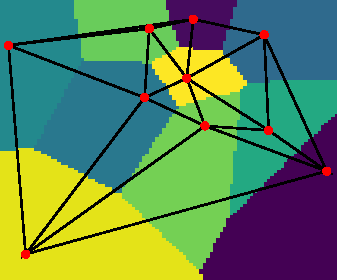
\includegraphics[width=0.29\textwidth]{img/chapitre3/figure4/nearest.pdf}}\hspace{1em}
    \subfigure[\label{fig-interpolation-b}Interpolation linéaire]{
        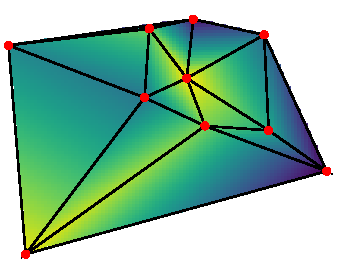
\includegraphics[width=0.29\textwidth]{img/chapitre3/figure4/linear.pdf}}\hspace{1em}
    \subfigure[\label{fig-interpolation-c}Interpolation cubique]{
        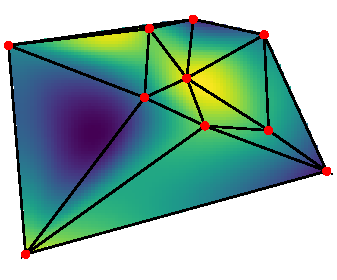
\includegraphics[width=0.29\textwidth]{img/chapitre3/figure4/cubic.pdf}}\\
    \subfigure[\label{fig-interpolation-d}\gls{ppv} - surface]{
        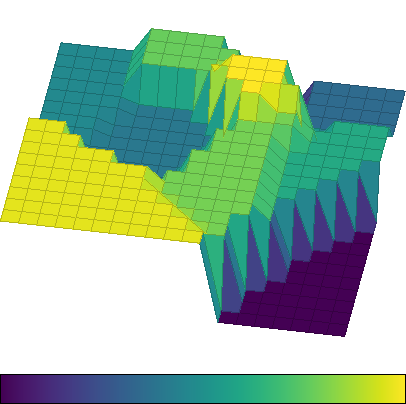
\includegraphics[width=0.29\textwidth]{img/chapitre3/figure4/surf_nearest.pdf}}\hspace{1em}
    \subfigure[\label{fig-interpolation-e}Interpolation linéaire - surface]{
        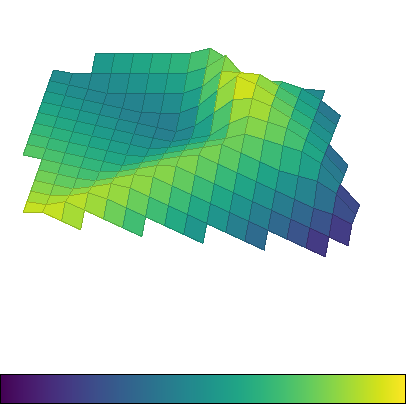
\includegraphics[width=0.29\textwidth]{img/chapitre3/figure4/surf_linear.pdf}}\hspace{1em}
    \subfigure[\label{fig-interpolation-f}Interpolation cubique - surface]{
        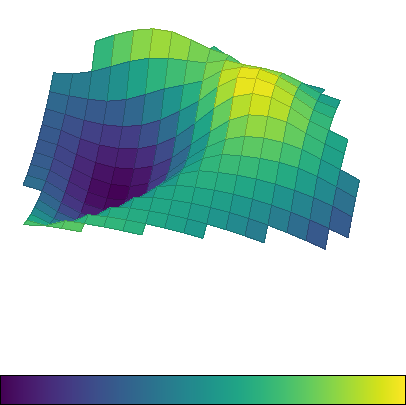
\includegraphics[width=0.29\textwidth]{img/chapitre3/figure4/surf_cubic.pdf}}
    \caption{Un ensemble de point (en rouge) est aléatoirement tiré et des valeurs leur sont associées. La triangulation de Delaunay est représentée en noire. La fonction est interpolée sur le carré unité. \protect\subref{fig-interpolation-a} Interpolation \gls{ppv}. \protect\subref{fig-interpolation-b} Interpolation bilinéaire. \protect\subref{fig-interpolation-c} Interpolation bicubique. Les fonctions interpolées sont également représentées dans le même ordre sous forme de surfaces aux figures~\subref{fig-interpolation-d} à \subref{fig-interpolation-f} (la résolution spatiale est diminuée pour des raisons d'affichage).
        \protect\label{fig-interpolation}}
\end{figure}

\paragraph{Avantages et inconvénients} Les méthodes d'interpolation ont pour principal avantage leur faible complexité et leur rapidité, ce qui en font des méthodes populaires en reconstruction en ligne~\cite{sibson1981interpreting, cazals2006delaunay, trampert2018ultramicroscopy}. Néanmoins, elles ne sont pas robustes puisqu'elles s'ajustent aux valeurs disponibles elles-mêmes corrompues. Elles ne permettent pas d'introduire plus d'information a priori que l'ordre de la fonction à interpoler.

\subsection{Les techniques de \glsentrylong{mc} régularisés}

Une approche \emph{variationelle} en inpainting est une méthode calculant l'image reconstruite en minimisant une fonction objectif appelée \emph{fonctionnelle}. En particulier, une technique de \gls{mc} régularisée fournit une image reconstruite \gls{Xh} en résolvant le problème de minimisation suivant~\cite[Section~6.3]{boyd2004convex}
\begin{equation}
    \gls{Xh} = \arg\min_{\gls{X}} \mathcal{L}(\gls{X}_{\gls{I}}, \gls{Y}) + \lambda \mathcal{R}(\gls{X})
\end{equation}
où $\mathcal{L}(\cdot, \gls{Y})$ est le terme d'attache aux données et où l'opérateur $\mathcal{R}$ est une régularisation. Le scalaire $\lambda$ permet d'ajuster l'importance de la régularisation par rapport au terme d'attache aux données. Cette formulation est liée à l'estimateur du maximum a posteriori puisque la formule de Bayes donne la fonction de vraisemblance $f(\gls{X}|\gls{Y}) \propto f(\gls{Y}|\gls{X}) f(\gls{X})$. En considérant l'opposé de la log-vraissemblance, l'estimée est l'image \gls{X} minimisant la fonction
\begin{equation}
    -\log f(\gls{X}|\gls{Y}) \propto
    \underbrace{-\log f(\gls{Y}|\gls{X})}_{\mathcal{L}(\gls{X}_{\gls{I}}, \gls{Y})}
    \underbrace{- \log f(\gls{X})}_{\mathcal{R}(\gls{X})}.
\end{equation}
Il en résulte que l'opérateur $\mathcal{L}$ est choisi en fonction du modèle statistique du bruit tandis que la régularisation dépend de l'information a priori disponible pour \gls{X}. Ces méthodes gèrent donc mieux la connaissance du bruit que les techniques d'interpolation et sont ainsi plus robustes. En particulier, le terme d'attache aux données pour un bruit additif gaussien blanc est une fonction coût quadratique $||\gls{Y}-\gls{X}_{\gls{I}}||_F^2$. Notons encore que les problèmes de \gls{mc} régularisés conviennent que l'information soit structurée ou non et qu'elles sont également utilisés pour la complétion en se basant sur une triangulation, comme c'est le cas en ajustement de surface~\cite{zhong2016surface,cazals2006delaunay}.

Un choix particulièrement classique pour la régularisation est la norme quadratique $\mathcal{R}(\gls{X}) = ||\gls{X}||_F^2$, on parle alors de régularisation de Tikhonov. L'avantage de cette forme est que la solution est  donnée par une expression mathématique directe, ne nécessitant qu'une inversion de matrice. La probabilité associée à \gls{X} est gaussienne centrée et promeut des données d'amplitude faible.

Les techniques de \gls{mc} régularisés sont également d'un intérêt particulier dans le cas de données  parcimonieuses, c'est-à-dire dont la proportion d'entrées non nulles est très faible. Dans ce cas, la régularisation idéale est la pseudo-norme $\ell_0$ \footnote{La pseudo-norme $\ell_0$ de \gls{X} vaut le nombre d'entrées non-nulle de \gls{X}. Il ne s'agit pas d'une norme puisque $||\alpha\gls{X}||_0 = ||\gls{X}||_0$ pour tout scalaire $\alpha$ non nul.} puisque celle-ci contraint le nombre d'éléments non-nuls. Malheureusement, résoudre ce problème d'estimation est très compliqué en pratique puisque la norme $\ell_0$ n'est pas faiblement convexe et on lui préfère généralement une relaxation convexe, comme la norme $\ell_1$ définie par $||\gls{X}||_1 = \sqrt{\sum |\gls{X}_i|}$. Cette méthode est souvent appelée Lasso~\cite{tibshirani1996regression} de l'acronyme \emph{Least Absolute Shrinkage and Selection Operator}. Enfin, il faut noter qu'utiliser la norme $\ell_1$ comme régularisation biaise le résultat. Pour corriger cela, des travaux ont proposé de résoudre le problème inverse en deux temps. D'abord, la technique Lasso est appliquée afin de déterminer les entrées non-nulles de l'estimée. Ensuite, une régression des moindres carrés est réalisée sur ce support. Cette méthode en deux temps est appelée post-LS (pour Least Square) ou encore \emph{refitting}~\cite{belloni2013least, lederer2013trust, deledalle2017clear}.

Utiliser la norme de $\gls{X}$ comme régularisation n'est pas toujours adaptée, en particulier lorsque le problème est sous-déterminé (i.e. où le nombre d'observations est inférieur au nombre de pixels). En effet, le terme d'attache aux données ne contraint pas les pixels manquants et en minimisant $||\gls{X}||$, ceux-xi prendraient des valeurs nulles. L'idée consistant à pénaliser les fortes valeurs prises par $\gls{X}$ peut être étendue de plusieurs façons. L'une d'entre elle consiste à pénaliser $\mathcal{A}\gls{X}$ où $\mathcal{A}$ est un opérateur linéaire. Ainsi, une alternative très populaire en traitement du signal consiste plutôt à pénaliser le gradient de l'image $\nabla\gls{X}$, conduisant à une régularisation $\mathcal{R}(\gls{X})=||\nabla\gls{X}||_F^2$, on parle aussi d'énergie de Sobolev. Le gradient est ainsi minimisé et une image lissée est restituée, comblant ainsi les régions sous-échantillonnées. De même, la régularisation $\ell_1$ peut être couplée avec un opérateur linéaire $\mathcal{A}$ pour favoriser la parcimonie du signal dans un cas particulier, par exemple :
\begin{itemize}
    \item si $\mathcal{A}$ est un changement de base telle que $\mathcal{A}\gls{X}$ soit parcimonieuse, la régularisation $||\mathcal{A}\gls{X}||_1$ est adaptée,
    \item si le gradient de l'image est calculée, la régularisation $||\nabla \gls{X}||_1$ appelée \gls{tv} promeut une image ayant peu de contours (l'image résultante est constante par morceaux).
\end{itemize}


\subsection{Les techniques par diffusion}

La diffusion est un processus physique très intuitif tendant à équilibrer les différences de concentration au sein d'un fluide sans créer ou détruire de masse. Ce phénomène est régi par l'équation de diffusion suivante
\begin{equation}
    \frac{\partial u}{\partial t} \triangleq \dot{u}(x, y, t) = \mathrm{div} (D(x, y)\cdot \nabla u)
\end{equation}
où $u$ est la concentration, $D$ est le coefficient de diffusion et $\nabla$ est l'opérateur gradient. En traitement de l'image, on identifie la concentration avec la valeur en niveau de gris prise en une position particulière. Si le coefficient de diffusion est constant sur toute l'image, on parle de diffusion \emph{isotropique} (ou linéaire), sinon, on parle de diffusion \emph{anisotropique} (ou non-linéaire).

La technique de diffusion la plus simple est la diffusion isotropique en débruitage, conduisant au problème aux dérivées partielles suivant
\begin{align}
&\dot{u} = D \cdot \Delta u\\
&u(\cdot, t=0) = y
\end{align}
où $y$ est l'image bruitée. Ce problème est équivalent à un filtrage avec un noyau gaussien d'écart-type $\sqrt{2t}$\footnote{L'image resultante en diffusion n'est pas l'image $u(\cdot, t=\infty)$ puisque celle-ci est constante (la diffusion tend à égaliser les niveaux de gris). Il faut choisir un instant $t^*$ où arrêter la trajectoire et l'image resultante est $u(\cdot, t^*)$.}~\cite{weickert1998anisotropic}. Le problème de cette technique est que la diffusion introduit un flou sur les contours de l'image. C'est pourquoi Perona et Malik~\cite{perona1990scale} ont proposé la diffusion anisotropique pour préserver les contours de l'image. Le coefficient de diffusion est diminué au niveau des contours tandis qu'il reste élevé au sein de zones homogènes. Le problème résultant s'écrit
\begin{align}
    &\dot{u}(x, y, t) = \mathrm{div} (D(|\nabla u|^2)\cdot \nabla u)\\
    & D(s) = \frac{1}{1+s^2/\lambda^2} \quad \text{pour $\lambda > 0$}
\end{align}

La technique de diffusion ne suffit cependant pas pour l'inpainting puisque la structure n'est pas propagée et un transport de matière doit être ajouté. Les travaux de Bertalmio \textit{et al.}~\cite{bertalmio2000image} ont été pionniers dans ce domaine et ont été à l'origine du terme \emph{inpainting}. S'inspirant des techniques de restauration en art, ils ont envisagé une technique par transport de matière propageant l'information le long de lignes de niveau (les lignes reliant les points de l'image ayant le même niveau de gris) dans le cas où celle-ci est structurée. Un terme de diffusion anisotropique était ajouté afin d'éviter que les lignes de niveau ne se croisent. D'autres techniqiues basée sur la variation totale on suivi~\cite{shen2002mathematical, chan2001nontexture} mais le principe fondamental consiste à propager la structure.

Ces techniques sont très bien adaptées aux images où l'information est très structurée, mais elles ne conviennent pas lorsque l'information est répartie. En effet, ces techniques reposent sur la propagation de contour. Dans le cas où les données sont réparties, aucun contour ne peut être propagé. C'est pourquoi nous n'utiliserons pas ces méthodes dans ce manuscrit.


\subsection{Les techniques par patch}

Une extension des méthodes variationelles exploite la redondance spatiale dans l'image, on parle alors de \emph{méthode par patch}. Elles constituent un ensemble de méthodes très populaires et performantes dont l'intérêt n'a cessé de grandir ces dernières décennies afin de résoudre des problèmes inverses comme le débruitage, l'inpainting ou la déconvolution.

Ces méthodes sont à opposer aux techniques dites \emph{locales} où une valeur est corrigée en ne la comparant qu'avec son voisinage, comme lorsqu'une image est convoluée avec un masque gaussien en débruitage. Le premier exemple de méthode \emph{non-locale} a été l'algorithme de débruitage Non-Local Mean~\cite{buades2005non} qui recherche des patchs semblables dans l'image afin de moyenner les pixels centraux. D'autres techniques plus évoluées en débruitage ont suivi, parmi lesquelles Block Matching and 3D filtering (BM3D)~\cite{dabov2007image} et Non Local Bayes~\cite{lebrun2013nonlocal}. Cependant, cette approche ne peux s'appliquer à l'inpainting seulement si l'information est structurée. Par exemple, l'algorithme \gls{ebi}~\cite{criminisi2004region} reconstruit des images partiellement corrompues en remplaçant de manière itérative les patchs manquants par le patch entier lui ressemblant le plus dans son voisinage. Des résultats ont également exprimés Non-Local Means sous forme variationelle, permettant ainsi des applications en reconstruction d'images dont l'information est répartie~\cite{peyre2008non, unni2018non, arias2009variational, yang2012nonlocal}.

Pour imposer la redondance spatiale, des algorithmes performants cherchent à représenter les patchs de l'image de manière parcimonieuse à l'aide d'\emph{atomes} contenus dans un \emph{dictionnaire}. Ces patchs caractéristiques sont appris conjointement aux données reconstruites, on parle alors de méthode par \gls{ad}. Une formulation générique de cette technique peut s'écrire comme le problème de \gls{mc} régularisé suivant~\cite{mairal2009online}
\begin{equation}
    \begin{aligned}
    (\mathbf{D}^*,\mathbf{A}^*) = &\arg\min_{(\mathbf{D}, \mathbf{A})}
    \frac{1}{2} || \mathbf{R}(\gls{Y}) - \mathbf{D A}||_F^2 + \lambda  || \mathbf{A} ||_1\\
    &\text{tel que } || \mathbf{D}_k ||_2 = 1 \quad \forall k\\
    \end{aligned}
\end{equation}
où $\mathbf{D}$ et $\mathbf{A}$ sont les matrices contenant respectivement les atomes et la décomposition parcimonieuse associé à chaque patch (on parle aussi de \emph{code}). $\mathbf{R}$, quant à lui, est l'opérateur permettant d'extraire les patchs des données et l'image reconstruite est obtenue par $\mathbf{R}^{-1}(\mathbf{D}^*\mathbf{A}^*)$. La contrainte permet de normaliser les atomes tandis que la régularisation $|| \mathbf{A} ||_1$ contraint le code à être parcimonieux. %
%
Cependant, la fonctionnelle à minimiser est non-convexe, rendant l'estimation conjointe du code et du dictionnaire compliqué, si bien que l'on préfère alterner le calcul du code et l'apprentissage du dictionnaire dont les formulations isolées sont convexes (mais le résultat est sous-optimal). C'est ainsi que l'algorithme de reconstruction wKSVD~\cite{mairal2008tip} alterne l'estimation des atomes par K-SVD~\cite{aharon2006k} et l'apprentissage du code par OMP~\cite{mallat1993matching, pati1993orthogonal} (la métrique de OMP est modifiée afin de mieux convenir aux images colorimétriques). L'algorithme ITKrMM~\cite{naumova2018fast, naumova2017dictionary} est un autre exemple d'algorithme fonctionnant sur ce principe, mais il a l'avantage d'être plus rapide puisqu'il estime le code à l'aide d'une opération de seuillage au lieu d'utiliser l'algorithme OMP plus lent. %
%
{\color{red}D'autres travaux proposent d'adopter une approche bayesienne afin d'estimer le code et le dictionnaire comme une densité de probabilité, l'algorithme très populaire en microscopie Beta-Process Factor Analysis (BPFA)~\cite{xing2012siam} initialement développé pour la reconstruction de données hyperspectrales. Ces techniques par \gls{ad} conviennent quelle que soit le type d'inpainting.}

Enfin, il faut bien mettre en avant que la reconstruction d'une image par \gls{ad} ne doit reposer sur les données corrompues \emph{uniquement}. Cette approche ne nécessitant aucune autre donnée est appelée \emph{méthode sans entraînement}. Cependant, il est aisé de reconstruire l'image dès lorsque le dictionnaire est disponible, si bien que les atomes sont parfois appris sur un jeu de données non-corrompues et utilisés ensuite pour la reconstruction, on parle alors de \emph{méthode par entraînement}. Cette approche est connue pour donner de bien meilleurs résultats, mais présente deux inconvénients majeurs :
\begin{itemize}
    \item cela nécessite un grand ensemble d'images propres (appelé données d'entraînement),
    \item le contenu spatial de l'image à reconstruire doit être similaire au contenu des données d'entraînement.
\end{itemize}
Les performances sont particulièrement dégradées si les structures sont différentes, tournées différemment ou d'échelle différente.



%
\section{Utilisation des techniques de reconstruction en microscopie}

Ce manuscrit se concentre sur la reconstruction d'images \gls{stem} spatialement sous-échantillonnées. Beaucoup de travaux ont étudié ce problème en employant différentes approches et modalités. Cette partie traite de ces travaux en les divisant en deux parties. La première considère les méthodes \emph{sans entraînement} qui reconstruisent les images à l'aide des seules données acquises. La seconde étudie les méthodes \emph{avec entraînement} qui s'appuient sur des données d'entraînement pour calibrer un opérateur utilisé ensuite en complétion de données.

\subsection{Méthodes sans entraînement}

L'interpolation \gls{ppv} est une solution simple et rapide, autorisant parfois de réaliser conjointement l'acquisition et la reconstruction en temps réel. Cependant, pour éviter que l'image reconstruite soit constante par morceau, on préfère pondérer les valeurs prises par les pixels voisins, comme expliqué à l'\cref{eq-weighted-interp}. La distance entre le pixel à interpoler et le voisin est inversée puis normalisée afin de former la pondération. Cette approche est utilisée en reconstruction d'images \gls{sem} dans~\cite{godaliyadda2018tci}, \gls{edx} dans~\cite{zhang2018reduced, hujsak2018high} et \gls{eels} dans~\cite{hujsak2018high}. L'interpolation par plus proches voisins naturels qui ajuste les poids en se basant sur une représentation de Voronoi est choisi comme alternative pour des images \gls{sem} dans~\cite{trampert2018ultramicroscopy}.

Les méthodes par \gls{mc} régularisés offrent généralement de meilleurs résultats que \gls{ppv} puisqu'elles contraignent l'image reconstruite à suivre un comportement prédéfini, généralement promue par une régularisation adaptée. Un choix classique puisque motivée par le paradigme de l'acquisition comprimée promeut la parcimonie dans une base adaptée, comme la régularisation $\ell_1$ utilisée pour des images de \gls{mfa} dans~\cite{han2018optimal}. Ce type de \gls{mc} régularisé sera noté $\ell_1-\gls{mc}$ dans le \cref{tab-litterature}. %
Dans le cas de structures périodiques (comme c'est le cas pour des images à échelle atomique), la base de Fourier ou la \gls{dct} peuvent être utilisées. Les auteurs de~\cite{stevens2018apl} ont ainsi proposé une méthode de reconstruction d'image \gls{haadf} reposant sur une transformée de Fourier seuillée, contraignant ainsi la parcimonie dans cette base périodique. La méthode proposée dans~\cite{beche2016development} utilise l'algorithme SPGL1~\cite{berg2008probing} afin de promouvoir la parcimonie dans la base \gls{dct} et reconstruire des images \gls{haadf}. De la même façon, cette régularisation peut être couplée avec une base d'ondelette pour reconstruire des images \gls{haadf} en ligne\cite{li2018compressed}. %
%
La régularisation \gls{tv} est aussi classiquement utilisée pour favoriser la reconstruction d'images constantes par morceaux, comme proposé en~\cite{han2018optimal} pour des données \gls{mfa}. La représentation \gls{dct} par block a été couplée avec la \gls{tv} en reconstruction d'images \gls{sem} dans~\cite{anderson2013sparse}.%



Les méthodes par patch offrent généralement de meilleurs performances puisqu'elles exploitent la redondance spatiale. En particulier, les techniques par \gls{ad} estiment conjointement les atomes constituant un dictionnaire et la représentation parcimonieuse associée. %
%
BPFA est très probablement la méthode par \gls{ad} la plus populaire dans la communauté de microscopie~\cite{xing2012siam}. Il a été appliqué pour la première fois sur des images \gls{haadf} à échelle atomique~\cite{stevens2013potential} et a été utilisé par la suite dans de nombreux travaux pour le même type de données~\cite{mucke2016practical,kovarik2016implementation}.
%
Les auteurs de BPFA ont également proposé la méthode Kruskal-factor analysis (KFA) comme une extension tensorielle de BPFA~\cite{stevens2017tensor}. KFA a été appliqué à la reconstruction d'images \gls{eels} en se basant sur une acquisition multiplexée d'un spectre-image~\cite{stevens2016mm}.
%
Enfin, l'algorithme EPLL (Expected-Patch Log-Likelihood) fait l'hypothèse que la distribution statistique des patchs suit un mélange de lois gaussiennes~\cite{zoran2011from}. Cependant, cet algorithme est particulièrement lent, si bien que les auteurs ont préférés une implémentation simplifiée mais accélérée appelée Fast EPLL (FEPLL) afin de reconstruire des images \gls{sem}~\cite{parameswaran2019accelerating}.
%
En plus des méthodes utilisée dans la communauté de microscopie, wKSVD~\cite{mairal2008tip} et ITKrMM~\cite{naumova2018fast,naumova2017dictionary} apprennent le dictionnaire à partir de données incomplètes sans faire d'hypothèse particulière sur la distribution des patchs. Il s'agit pourtant de méthodes de l'état de l'art et elles seront considéré dans la suite de l'étude.

Afin d'atteindre de meilleures performances avec une dose d'électron réduite, plusieurs chemins d'acquisition ont été proposés, comme l'échantillonnage aléatoire de lignes horizontales~\cite{kovarik2016implementation,han2018optimal}, l'échantillonnage mixe régulier-aléatoire~\cite{stevens2018apl}, les chemins en spirale~\cite{sang2017dynamic,li2018compressive,han2018optimal} ou enfin les chemins en forme de carré~\cite{han2018optimal}.
%
Ces résultats tendent à montrer que les performances optimales sont atteintes par des acquisitions semi-aléatoires, qui introduisent de l'aléatoire dans des structures régulières, ce qui évite les grands trous. %
%
Finalement, des améliorations conséquentes en reconstruction ont été rendus possibles par l'acquisition adaptative qui sélectionne le pixel à échantillonner à partir des données précédemment acquises. Dans~\cite{dahmen2016feature}, les auteurs proposent de faire un premier échantillonnage à bas SNR afin de localiser les contours de l'image. Une seconde acquisition à SNR élevé est ensuite effectuée sur ces contours seulement. Enfin, les parties lisses de la première image sont filtrées tandis que les contours sont remplis avec les pixels issues de la seconde acquisition. Un schéma d'acquisition adaptative alternatif proposé dans~\cite{dahmen2019adaptive} consiste à localiser de manière itérative des points d'intérêt à échantillonner. Les techniques d'acquisition adaptatives partielles avec entraînement sont présentées à la sous-section suivante.

\subsection{Méthodes avec entraînement}

Contrairement aux méthodes sans apprentissage qui reconstruisent l'image complète à partir des seules données acquises, les méthodes avec entraînement apprennent un opérateur en exploitant des données d'entraînement. Par exemple, l'algorithme GOAL apprend un dictionnaire en maximisant la parcimonie de la représentation des données d'apprentissage~\cite{hawe2013analysis}. Le dictionnaire estimé est ensuite utilisé afin de reconstruire les données de test. De manière similaire, EBI qui est initialement une technique sans apprentissage peut être adapté afin de tirer parti de données d'apprentissage. Pour cela, au lieu d'extraire le patch à copier du voisinage, comme c'est le cas dans l'implémentation conventionnelle de EBI, ce patch est choisi parmi un dictionnaire appris auparavant sur des images non-corrompues. Cette stratégie est suivie dans~\cite{trampert2018exemplar} pour reconstruire des données 3D en \gls{sem}. GOAL et la version avec apprentissage de EBI ont été appliqués dans~\cite{trampert2018ultramicroscopy} pour des images 2D en \gls{sem}, mais BPFA semblait donner de meilleurs résultats.

Les approches avec apprentissage peuvent aussi être envisagée afin de décider quelle position devrait être échantillonnée pour minimiser la distorsion après reconstruction. En effet, la position des pixels échantillonnés impacte grandement la qualité de la reconstruction lorsque les données sont sous-échantillonnées~\cite{trampert2018ultramicroscopy}. Pour améliorer cette qualité, l'algorithme SLADS (supervised learning approach for dynamic sampling) apprend une fonction (appelée réduction de distorsion espérée (RDE)) indiquant quelle position devrait être échantillonnée afin de réduire la distorsion au maximum\cite{godaliyadda2018tci}. Cette étape d'apprentissage repose sur une liste de caractéristiques et sur des données labellisées et a été utilisée pour dynamiquement échantillonner des images \gls{sem}.
%
Cette méthode a aussi été appliquée à des données \gls{edx} dans~\cite{zhang2018reduced}. Pour cela, un réseau de neurones convolutif classifie les spectres des données test et la fonction RDE est calculée simultanément pour tous les labels. %
%
Le papier~\cite{hujsak2018high} a ensuite modifié cette approche pour permettre des mélanges d'éléments en \gls{eels} et en \gls{edx}. Toutes ces approches requirent une technique de reconstruction rapide et l'interpolation pondérée \gls{ppv} a été utilisée.



%
\section{Motivations et contribution}

Dans cette étude, nous envisageons le schéma d'acquisition partielle afin de préserver l'échantillon en microscopie \gls{stem}-\gls{eels}. En particulier, une motivation consiste à réduire le temps de calcul associé à l'étape d'inpainting en vue de l'insérer dans un processus d'acquisition. L'expérimentateur devrait être capable de visualiser le spectre-image complet au cours de l'acquisition, ce qui requiert à la fois un temps de calcul réduit et une bonne précision. En plus de ce processus en ligne, l'expérimentateur devrait être capable de raffiner le spectre-image reconstruit a posteriori. Dans ces conditions, des algorithmes plus précis mais nécessitant plus de temps de calcul sont autorisés. 

\begin{table*}[t]
    \centering
    \bgroup
    \renewcommand{\arraystretch}{1.2}
    \begin{tabular}{>{\arraybackslash\centering}m{3cm}*{5}{c}}
        \toprule
        \multirow{2}*{Famille}& \multirow{2}*{Méthode}& \multicolumn{2}{c}{Travaux}& 
        \multirow{2}*{Temps d'exécution}& \multirow{2}*{Précision}\\
        %
        &&2D&3D&&\\
        %
        \midrule
        %
        \multirow{2}*{Interpolation} & \gls{ppv} & - & - & \plusfa[3] & \minusfa[2]\\
        %
        & Voisinage pondéré & \cite{sibson1981interpreting, cazals2006delaunay, trampert2018ultramicroscopy}&
        - & \plusfa[2] & \minusfa[1]\\
        %
        \midrule
        %
        \multirow{4}*{\gls{mc}-régularisé}&
        $\ell_1$-\gls{mc} & \cite{han2018optimal,beche2016development,li2018compressed,anderson2013sparse}&
        & \plusfa & \plusfa\\
        %
        & TV-\gls{mc} & \cite{han2018optimal} & - & \plusfa[1] & \plusfa\\
        %
        %
        \midrule
        %
        \multirow{6}{3cm}{\centering Méthode par \gls{ad}}&
        BPFA & {\cite{stevens2013potential,trampert2018ultramicroscopy}} &
        \textit{\cite{xing2012siam}} & \minusfa[3] & \plusfa[3]\\
        %
        & EBI & \cite{trampert2018ultramicroscopy} & {\cite{trampert2018exemplar}} &
        \minusfa[1] & \plusfa[2]\\
        %
        & FEPLL & \textit{\cite{parameswaran2019accelerating}},\cite{hujsak2018high} &
        - & \minusfa[1] & \plusfa[2]\\
        %
        & wKSVD & - & \textit{\cite{mairal2008tip}} & \minusfa[2] & \plusfa[2]\\
        %
        &
        ITKrMM & \textit{\cite{naumova2018fast}} & \textit{\cite{naumova2017dictionary}}&
        \minusfa[1] & \plusfa[2]\\
        %
        & GOAL & \textit{\cite{hawe2013analysis}},\cite{trampert2018ultramicroscopy}&
        - & \minusfa[1] & \plusfa[2]\\
        %
        \bottomrule
    \end{tabular}
    \egroup
    \caption{Comparaison des méthodes proposées dans la littérature en microscopie pour le reconstruction d'images partiellement échantillonnées. Des références supplémentaires n'étant pas issues de la littérature en microscopie sont données en italique. Le temps d'exécution et la précision sont évaluées qualitativement en se basant sur les résultats des chapitres suivants.%
        \protect\label{tab-litterature}}
\end{table*}

Afin de déterminer l'approche à privilégier, le \cref{tab-litterature} résume l'état de l'art en microscopie réalisé dans la section précédente Les méthodes y sont notées en fonction de leur complexité et de leur précision et groupées selon trois grandes familles : l'interpollation, les \gls{mc} regularisés et les méthodes par \gls{ad}. Pour chaque méthode, les travaux issus de la littérature sont fournis et séparés selon que les données reconstruites soient des images 2D mono-bandes (e.g. \gls{haadf}) ou des spectre-images 3D (e.g. \gls{eels}).

Parmi les méthodes compatibles avec les données \gls{eels}, \gls{ppv} est rapide mais les performances en reconstruction sont généralement mauvaises tandis que les méthodes par \gls{ad} sont très efficaces mais sont très lourdes en temps de calcul, tout particulièrement lorsque des patchs 3D sont appris. Par conséquent, cet état de l'art met en évidence une lacune : aucune technique disponible peut reconstruire précisément un spectre-image spatialement sous-échantillonné suffisamment rapidement pour l'inclure dans un processus expérimental d'acquisition en ligne. D'autant que l'acquisition et la reconstruction rapide d'un spectre-image \gls{eels} n'a suscité que peu d'intérêt en comparaison de sa contrepartie hyperspectrale en observation de la Terre~\cite{zhang_hyperspectral_2014, chayes_pre_processing_2017, golbabaee_hyperspectral_2012, chen_inpainting_2012}.

Une alternative pour systématiquement reconstruire un spectre-image consiste à traiter les images 2D associés à chaque canal \emph{séparément} et \emph{en parrallèle}. Notons d'ailleurs que \gls{ppv} fonctionne de cette façon lorsqu'il reconstruit un spectre-image spatialement sous-échantillonné. Cependant, cette approche est sous-optimale puisque la tâche de reconstruction est censée être plus efficace en s'appuyant sur les données 3D complètes. Des stratégies similaires consisteraient à ne reconstruire que les images associées à un ou plusieurs canaux d'intérêt nécessaires pour la cartographie d'éléments. Cependant, cette approche serait aussi sous-optimale quand aucun a priori serait disponible concernant l'échantillon à observer.

Pour conclure, ni l'interpolation \gls{ppv}, ni les méthodes par \gls{ad} ne sont adaptés à la reconstruction précise en ligne et seulement les méthodes par \gls{mc} allient précision et charge calculatoire réduite. C'est donc ce type d'approche qui a été étudié dans la suite de ce manuscrit. Et puisque les performances des méthodes par \gls{mc} régularisés dépendent fortement de l'information disponible a priori, la reconstruction d'images \gls{eels} en basse résolution sera étudiée dans le \cref{ch-chapter_3} tandis que les images haute résolution le seront dans le \cref{ch-chapter_4}. Remarquons finalement que les méthodes par \gls{ad} sont les techniques les plus performantes disponibles et qu'elles conviennent parfaitement à l'étape de raffinement effectuée hors processus d'acquisition. Ces techniques particulièrement performantes ne seront pas étudiées par la suite (bien qune approche non-locale régularisée ait été envisagée) et ne servirons que de comparaison aux approches proposées.



